\documentclass[12pt, a4paper, oneside]{book}
\usepackage[hidelinks]{hyperref}
\usepackage[slovak,english]{babel}
\usepackage{epsfig}
\usepackage{epstopdf}
\usepackage{makecell}
\usepackage{lineno}
\usepackage{algorithm}
\usepackage{algpseudocode}
\usepackage{algorithmicx}
\usepackage{multirow}
\usepackage{listings}
\usepackage{lscape}
\usepackage{amsmath}
\usepackage{mathtools}
\usepackage{amssymb}
\usepackage{graphicx}
\usepackage{multirow}
\usepackage{color}
\usepackage{url}
\usepackage{setspace}
\usepackage{tabularx}
\usepackage{textcomp}
\usepackage{caption}
\usepackage{natbib}
\usepackage{float}
\usepackage{xcolor}
\usepackage{appendix}

\usepackage[T1]{fontenc}
\usepackage{lmodern}

\makeatletter
\newcommand{\algmargin}{\the\ALG@thistlm}
\makeatother
\algnewcommand{\parState}[1]{\State%
\parbox[t]{\dimexpr\linewidth-\algmargin}{\strut\hangindent=\algorithmicindent \hangafter=1 #1\strut}}

\newcommand\todo[1]{\textcolor{red}{#1}}
\newtheorem{definition}{Definition}
\newtheorem{theorem}{Theorem}
\numberwithin{definition}{chapter}
\numberwithin{theorem}{chapter}

\setstretch{1.5}
%\renewcommand\baselinestretch{1.5} % riadkovanie jeden a pol

% pekne pokope definujeme potrebne udaje
\newcommand\mftitle{Symmetries of Combinatorial Structures}
\newcommand\mfthesistype{Diploma Thesis}
\newcommand\mfauthor{Bc. Matúš Gál}
\newcommand\mfadvisor{doc. RNDr. Tatiana Jajcayová, PhD.}
\newcommand\mfplacedate{Bratislava, 2023}
\newcommand\mfuniversity{COMENIUS UNIVERSITY IN BRATISLAVA}
\newcommand\mffaculty{FACULTY OF MATHEMATICS, PHYSICS AND INFORMATICS}
\newcommand{\sub}[1]{$_{\text{#1}}$}
\newcommand{\reference}[1]{č.~\ref{#1}}
\newcommand{\imageHeight}{150px}

\ifx\pdfoutput\undefined\relax\else\pdfinfo{ /Title (\mftitle) /Author (\mfauthor) /Creator (PDFLaTeX) } \fi

\begin{document}
\frontmatter

\thispagestyle{empty}

\noindent
\begin{minipage}{\textwidth}
\begin{center}
\textbf{\mfuniversity \\
\mffaculty}
\end{center}
\end{minipage}

\vfill
\begin{figure}[!hbt]
\begin{center}

\includegraphics{images/new_logo}
%
\includegraphics{images/new_logo.png}
%\label{img:logo}
\end{center}
\end{figure}
\begin{center}
\begin{minipage}{0.8\textwidth}
\centerline{\textbf{\Large\MakeUppercase{\mftitle}}}
\smallskip
\centerline{\mfthesistype}
\end{minipage}
\end{center}
\vfill
2023 \hfill
\mfauthor
\eject
% koniec obalu

%\thispagestyle{empty}
%\newpage
%\
%\newpage
\thispagestyle{empty}

\noindent
\begin{minipage}{\textwidth}
\begin{center}
\textbf{\mfuniversity \\
\mffaculty}
\end{center}
\end{minipage}

\vfill
\begin{figure}[!hbt]
\begin{center}

\includegraphics{images/new_logo}
%\label{img:logo_dark}
\end{center}
\end{figure}
\begin{center}
\begin{minipage}{0.8\textwidth}
\centerline{\textbf{\Large\MakeUppercase{\mftitle}}}
\smallskip
\centerline{\mfthesistype}
\end{minipage}
\end{center}
\vfill
\begin{tabular}{l l}
%Registration number: & 40a99bd8-3cb6-4534-9330-c7fd9b5e5ca4 \\
Study Programme: & Applied Informatics \\
Field of Study: & 2508 Informatics \\
Department: & Department of Applied Informatics\\
Supervisor: & \mfadvisor
\end{tabular}
\vfill
\noindent
\mfplacedate \hfill
\mfauthor
\eject
% koniec titulneho listu

%\thispagestyle{empty}
%\includegraphics[width=\textwidth]{images/zadanie}
%\vfill
%\eject
% koniec zadania

%\thispagestyle{empty}
%\newpage
%\
%\newpage
\thispagestyle{empty}

\begin{figure}[H]
\begin{center}
\makebox[\textwidth]{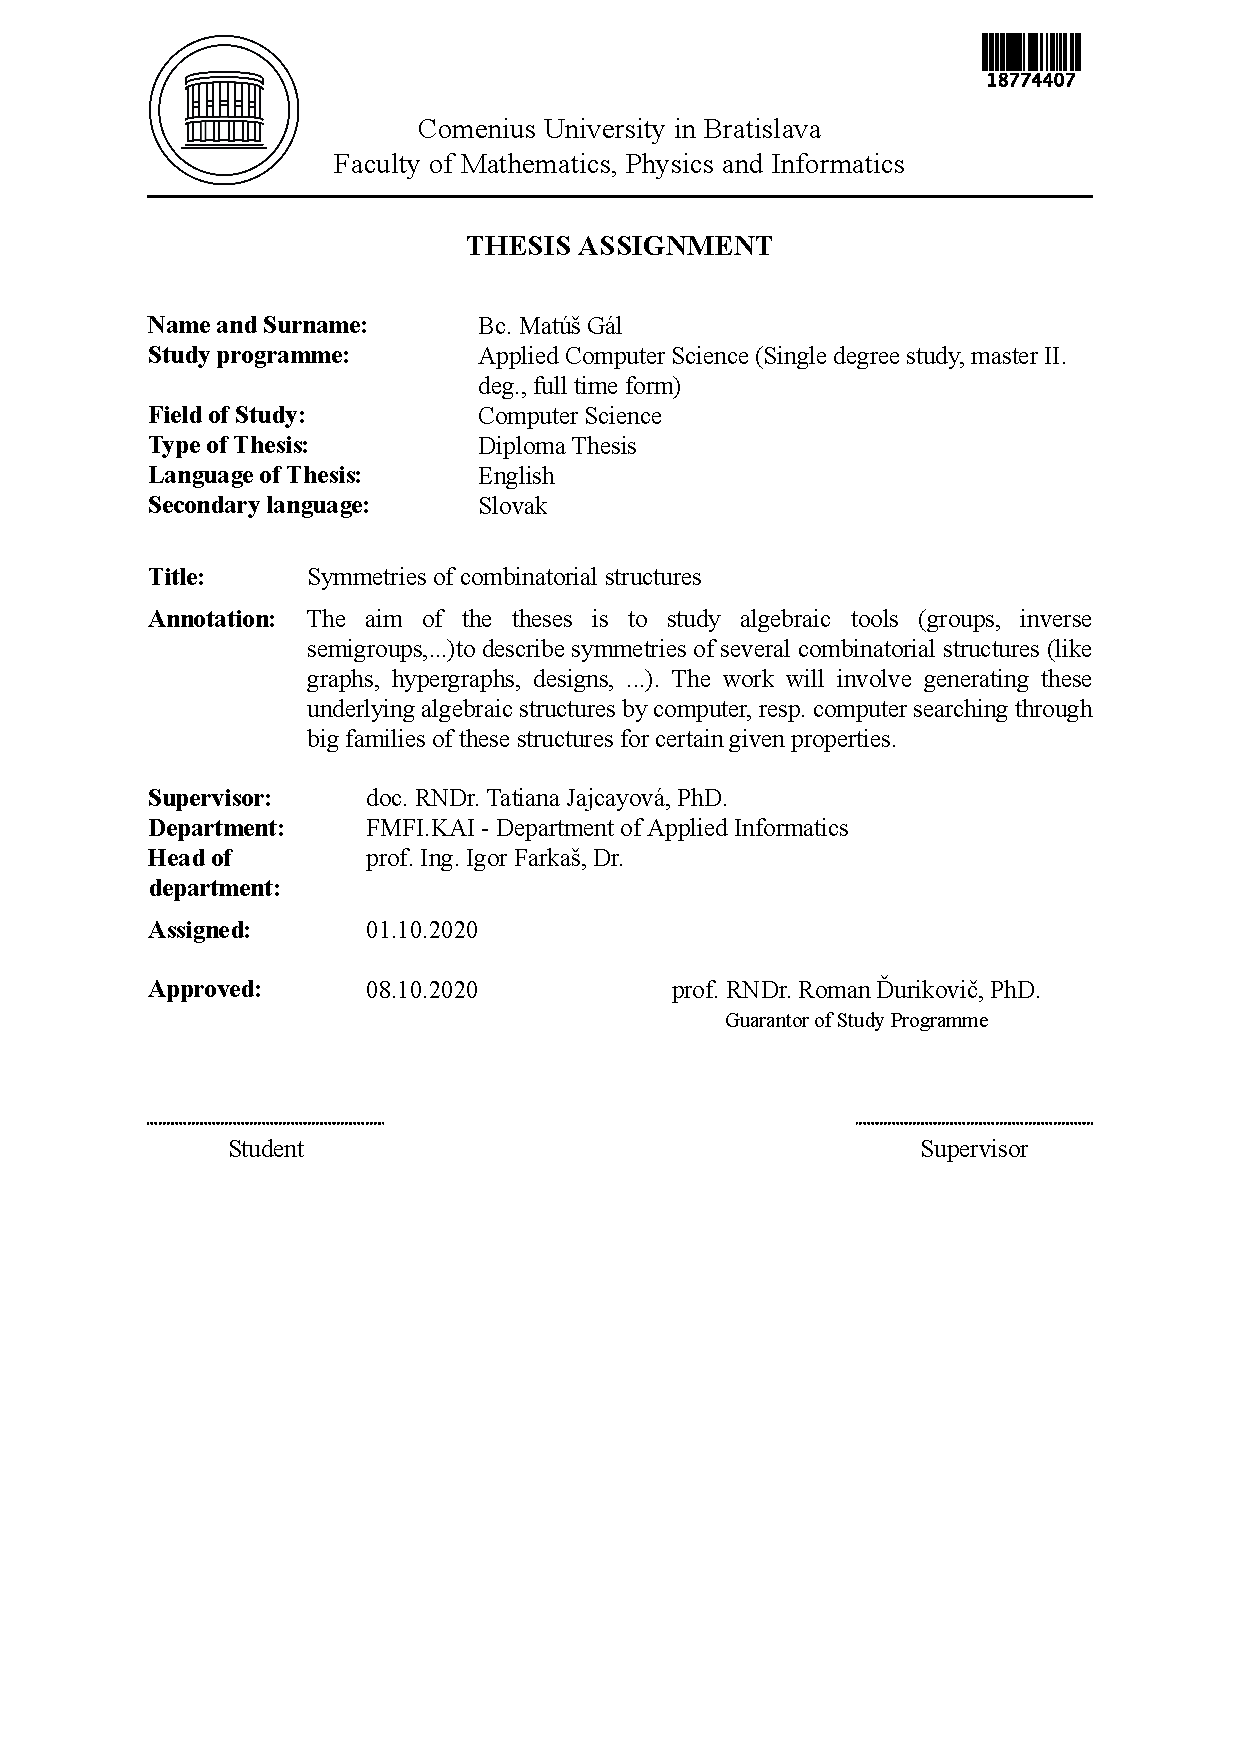
\includegraphics[width=\paperwidth]{images/zadanie_en.pdf}}
\label{img:zadanie}
\end{center}
\end{figure}

{~}\vspace{12cm}

\noindent
\begin{minipage}{0.25\textwidth}~\end{minipage}
\begin{minipage}{0.75\textwidth}
Hereby I declare I worked on this thesis on my own, using the sources listed in the bibliography and under the supervision of my thesis supervisor.
\newline \newline
\end{minipage}
\vfill
~ \hfill {\hbox to 6cm{\dotfill}} \\
\mfplacedate \hfill \mfauthor
\vfill\eject
% koniec prehlasenia

\chapter*{Acknowledgements}\label{chap:thank_you}
Firstly, I would like to thank my thesis supervisor doc. RNDr. Tatiana Jajcayová, PhD., for her help in making complex topics easy to understand and providing feedback.

I also want to thank everyone who mentally supported me and kept me going throughout the writing of this thesis.
\vfill\eject
% koniec podakovania
\vfill\eject

\chapter*{Abstract}\label{chap:abstract_en}

The aim of this thesis is to study both the symmetries and partial symmetries of graphs and explore them using algebraic tools from group theory and inverse semigroup theory.

When studying symmetries of graphs using groups, one quickly finds this approach is insufficient, since almost all graphs are asymmetric, meaning they have no non-trivial symmetries. For this reason, we need to use tools from inverse semigroup theory, such as inverse monoids and Green's relations, to examine partial symmetries of graphs, specifically the symmetries between their vertex-induced subgraphs.

While our primary goal was studying the partial symmetries of minimal asymmetric graphs, our solution works with any graph. To find the inverse automorphism monoids of graphs we implemented an application in Python, which provides an interface for working with graphs, their full and partial automorphisms. With our algorithm, we achieved significantly better performance in comparison to other currently existing solutions.

Finally, we introduced the definition of asymmetric depth, used to measure the asymmetricity of graphs.

~\\
Keywords: graph theory, group theory, inverse semigroup theory, automorphism, partial automorphism
\vfill\eject
\chapter*{Abstrakt}\label{chap:abstract_sk}

Cieľom tejto diplomovej práce bolo štúdium symetrií a čiastočných symetrií grafov a ich skúmanie použitím algebraických nástrojov z teórie grúp a teórie inverzných pologrúp.

Pri štúdiu grafov použitím grúp zistíme, že tento prístup je neadekvátny vo väčšine prípadov, keďže takmer všetky grafy sú asymetrické, teda nemajú netriviálne symetrie. Z toho dôvodu potrebujeme použiť nástroje z teórie inverzných pologrúp, inverzné monoidy a Greenove relácie, na štúdium symetrií ich indukovaných podgrafov.

Našim primárnym cieľom bolo skúmanie čiastočných symetrií minimálnych asymetrických grafov, avšak naše riešenie je vhodné pre ľubovoľné grafy. Na nájdenie inverzných monoidov automorfizmov grafov sme implementovali aplikáciu v Pythone, ktorá ponúka rozhranie na prácu s grafmi, ich úplnými a čiastočnými symetriami. S našim algoritmom sme dosiahli lepšie výsledky ako ostatné aktuálne existujúce riešenia.

Nakoniec sme predstavili definíciu asymetrickej hĺbky, ktorá môže byť použitá na meranie asymetrickosti grafov.

~\\
Kľúčové slová: teória grafov, teória grúp, teória inverzných pologrúp, automorfizmus, čiastočný automorfizmus
% koniec abstraktov

\tableofcontents

\listoffigures
\listoftables

\mainmatter

% treba este prejst dokument ci je kod spravne formatovany
\input 01intro.tex
\input 02preliminaries.tex
\input 06implementation.tex
\input 07results.tex
\input 08conclusion.tex

\backmatter

\nocite{*}
\bibliographystyle{alpha}
\bibliography{references}

\begin{appendices}
\renewcommand\chaptername{Appendix}
\chapter*{Appendix}
\addcontentsline{toc}{chapter}{Appendix}
\label{ch:appendix}
\renewcommand{\thesection}{A.\arabic{section}}
\renewcommand{\thefigure}{A.\arabic{figure}}
\setcounter{figure}{0}
\setcounter{section}{0}
\markboth{APPENDIX}{APPENDIX}

We use the following notation for groups:

\begin{itemize}
\item $D_n$ - dihedral group of order $n$,
\item $S_n$ - symmetric group of degree $n$,
\item $C_n$ - cyclic group of order $n$,
\item $G x H$ - direct product of groups $G$ and $H$
\end{itemize}

\section{Partial automorphism monoid of minimal asymmetric graph X1}

\begin{figure}[H]
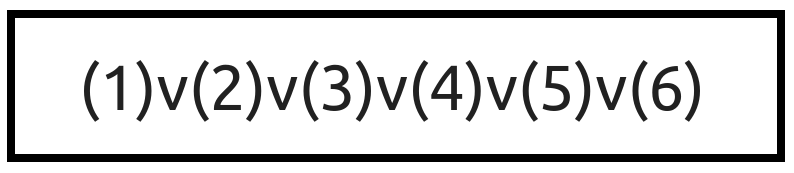
\includegraphics[scale=0.12]{images/x1/x1_6v_6e.png}
\caption{$\mathcal{D}$-class of induced subgraph with 6 vertices and 6 edges.}
\end{figure}

\begin{figure}[H]
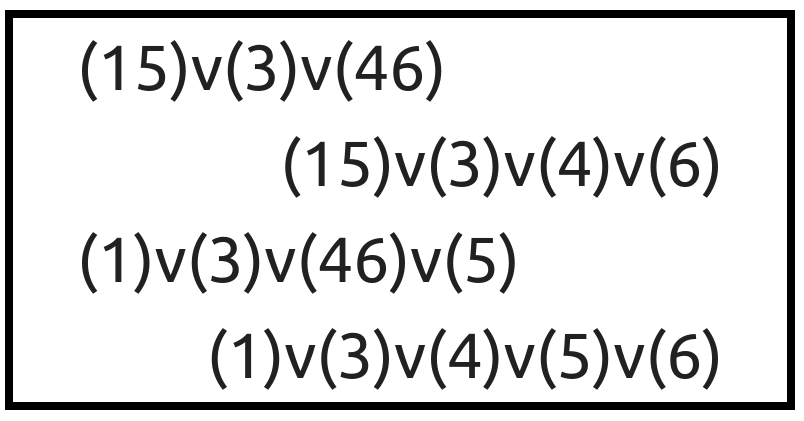
\includegraphics[scale=0.1]{images/x1/x1_5v_3e_2.png}
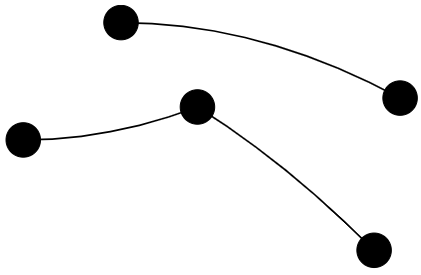
\includegraphics[scale=0.15]{images/x1/x1_5v_3e_2_vis.png}
\caption{$\mathcal{D}$-class of induced subgraph with 5 vertices and 3 edges (group C2xC2).}
\end{figure}

\begin{figure}[H]
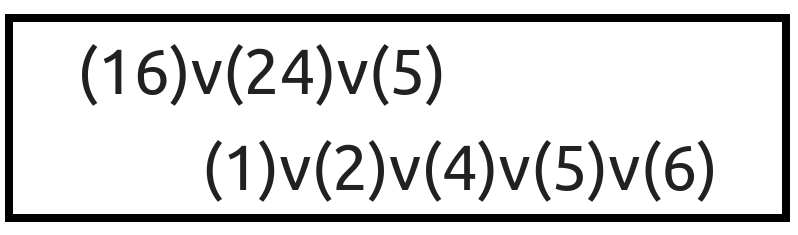
\includegraphics[scale=0.12]{images/x1/x1_5v_3e.png}
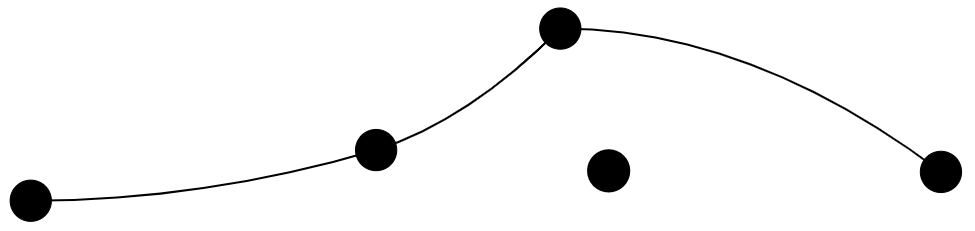
\includegraphics[scale=0.12]{images/x1/x1_5v_3e_1_vis.png}
\caption{$\mathcal{D}$-class of induced subgraph with 5 vertices and 3 edges (group C2).}
\end{figure}

\begin{figure}[H]
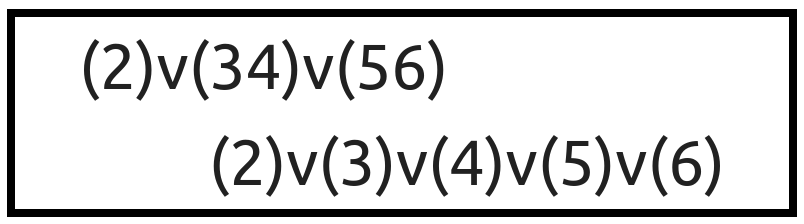
\includegraphics[scale=0.12]{images/x1/x1_5v_4e_2.png}
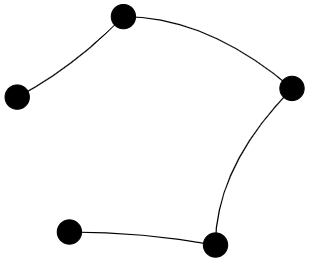
\includegraphics[scale=0.1]{images/x1/x1_5v_4e_2_vis.png}
\caption{$\mathcal{D}$-class of induced subgraph with 5 vertices and 4 edges (group C2).}
\end{figure}

\begin{figure}[H]
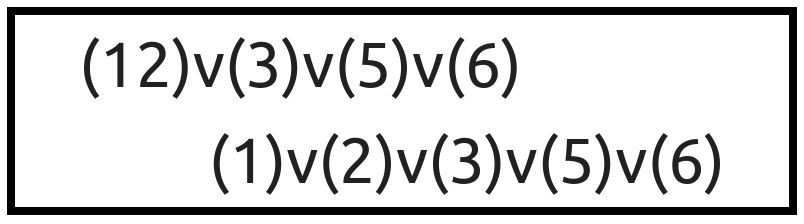
\includegraphics[scale=0.12]{images/x1/x1_5v_4e.png}
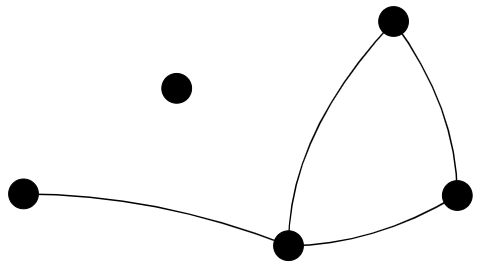
\includegraphics[scale=0.1]{images/x1/x1_5v_4e_1_vis.png}
\caption{$\mathcal{D}$-class of induced subgraph with 5 vertices and 4 edges (group C2).}
\end{figure}

\begin{figure}[H]
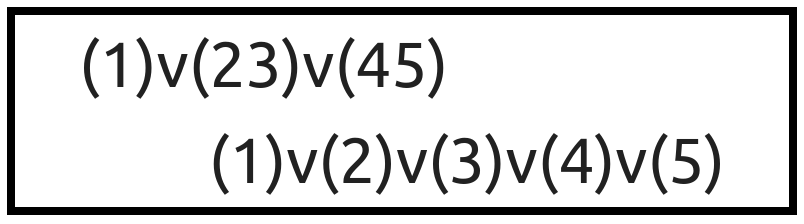
\includegraphics[scale=0.12]{images/x1/x1_5v_5e_2.png}
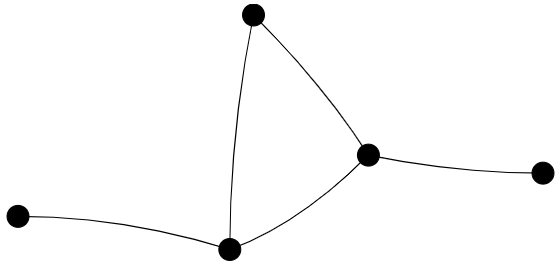
\includegraphics[scale=0.1]{images/x1/x1_5v_5e_2_vis.png}
\caption{$\mathcal{D}$-class of induced subgraph with 5 vertices and 5 edges (group C2).}
\end{figure}

\begin{figure}[H]
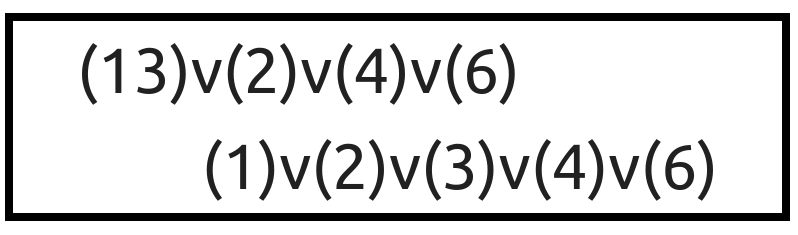
\includegraphics[scale=0.12]{images/x1/x1_5v_5e.png}
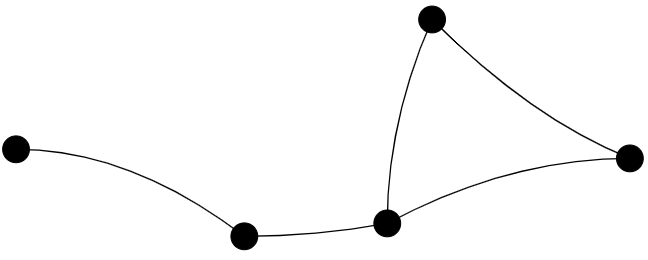
\includegraphics[scale=0.1]{images/x1/x1_5v_5e_1_vis.png}
\caption{$\mathcal{D}$-class of induced subgraph with 5 vertices and 5 edges (group C2).}
\end{figure}

\begin{figure}[H]
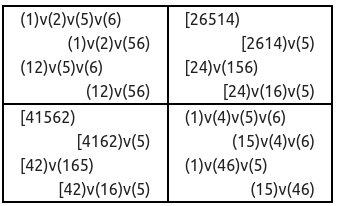
\includegraphics[scale=0.3]{images/x1/x1_4v_1e.png}
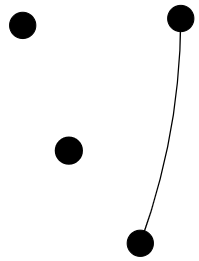
\includegraphics[scale=0.2]{images/x1/x1_4v_1e_vis.png}
\caption{$\mathcal{D}$-class of induced subgraph with 4 vertices and 1 edge (subgroup C2xC2).}
\end{figure}

\begin{figure}[H]
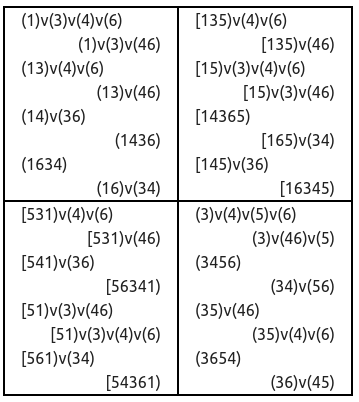
\includegraphics[scale=0.25]{images/x1/x1_4v_2e_2.png}
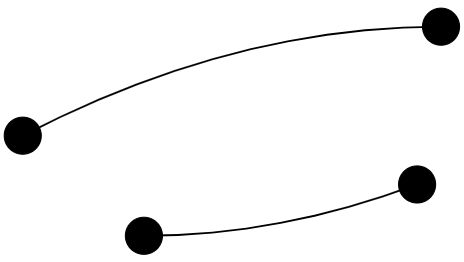
\includegraphics[scale=0.2]{images/x1/x1_4v_2e_2_vis.png}
\caption{$\mathcal{D}$-class of induced subgraph with 4 vertices and 2 edges (subgroup D8).}
\end{figure}

\begin{figure}[H]
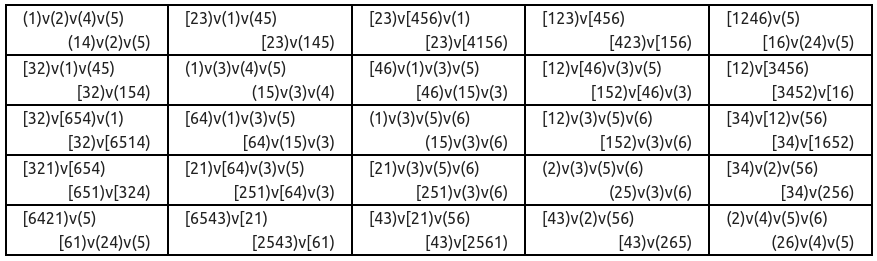
\includegraphics[scale=0.25]{images/x1/x1_4v_2e.png}
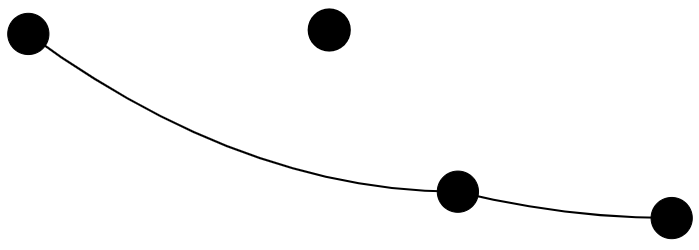
\includegraphics[scale=0.12]{images/x1/x1_4v_2e_1_vis.png}
\caption{$\mathcal{D}$-class of induced subgraph with 4 vertices and 2 edges (subgroup C2).}
\end{figure}

\begin{figure}[H]
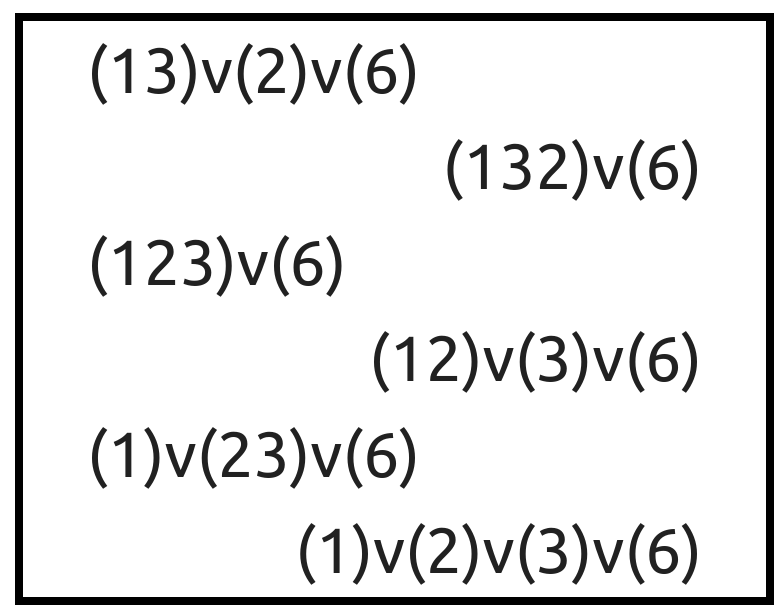
\includegraphics[scale=0.08]{images/x1/x1_4v_3e.png}
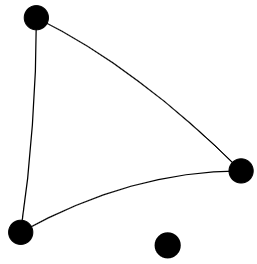
\includegraphics[scale=0.2]{images/x1/x1_4v_3e_1_vis.png}
\caption{$\mathcal{D}$-class of induced subgraph with 4 vertices and 3 edges (group S3).}
\end{figure}

\begin{figure}[H]
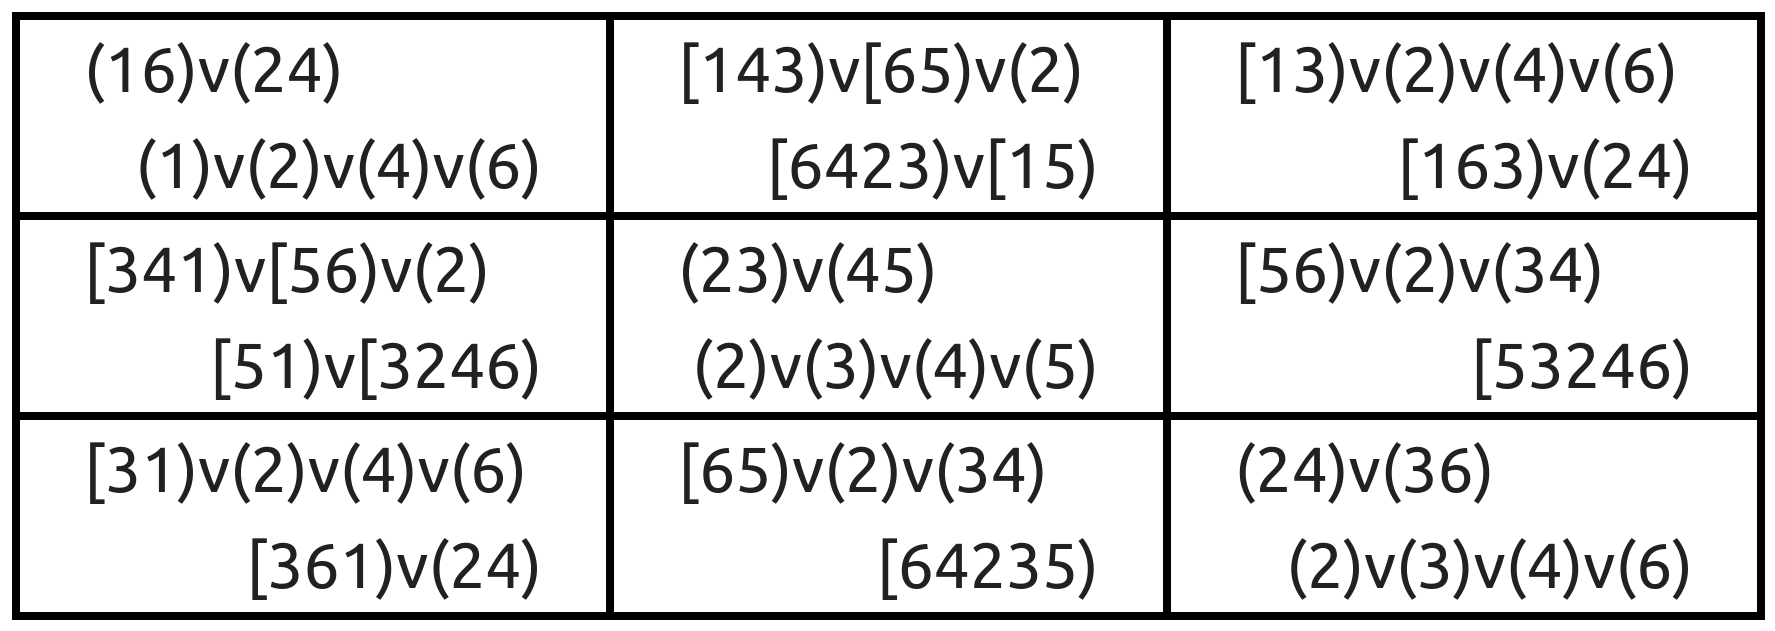
\includegraphics[scale=0.08]{images/x1/x1_4v_3e_2.png}
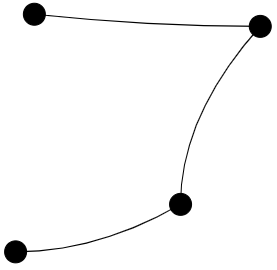
\includegraphics[scale=0.2]{images/x1/x1_4v_3e_2_vis.png}
\caption{$\mathcal{D}$-class of induced subgraph with 4 vertices and 3 edges (subgroup C2).}
\end{figure}

\begin{figure}[H]
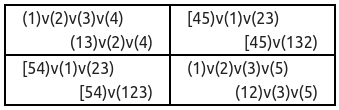
\includegraphics[scale=0.3]{images/x1/x1_4v_4e.png}
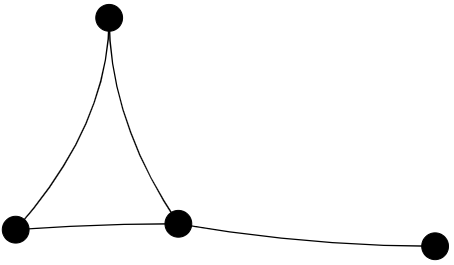
\includegraphics[scale=0.17]{images/x1/x1_4v_4e_vis.png}
\caption{$\mathcal{D}$-class of induced subgraph with 4 vertices and 4 edges (subgroup C2).}
\end{figure}

\begin{figure}[H]
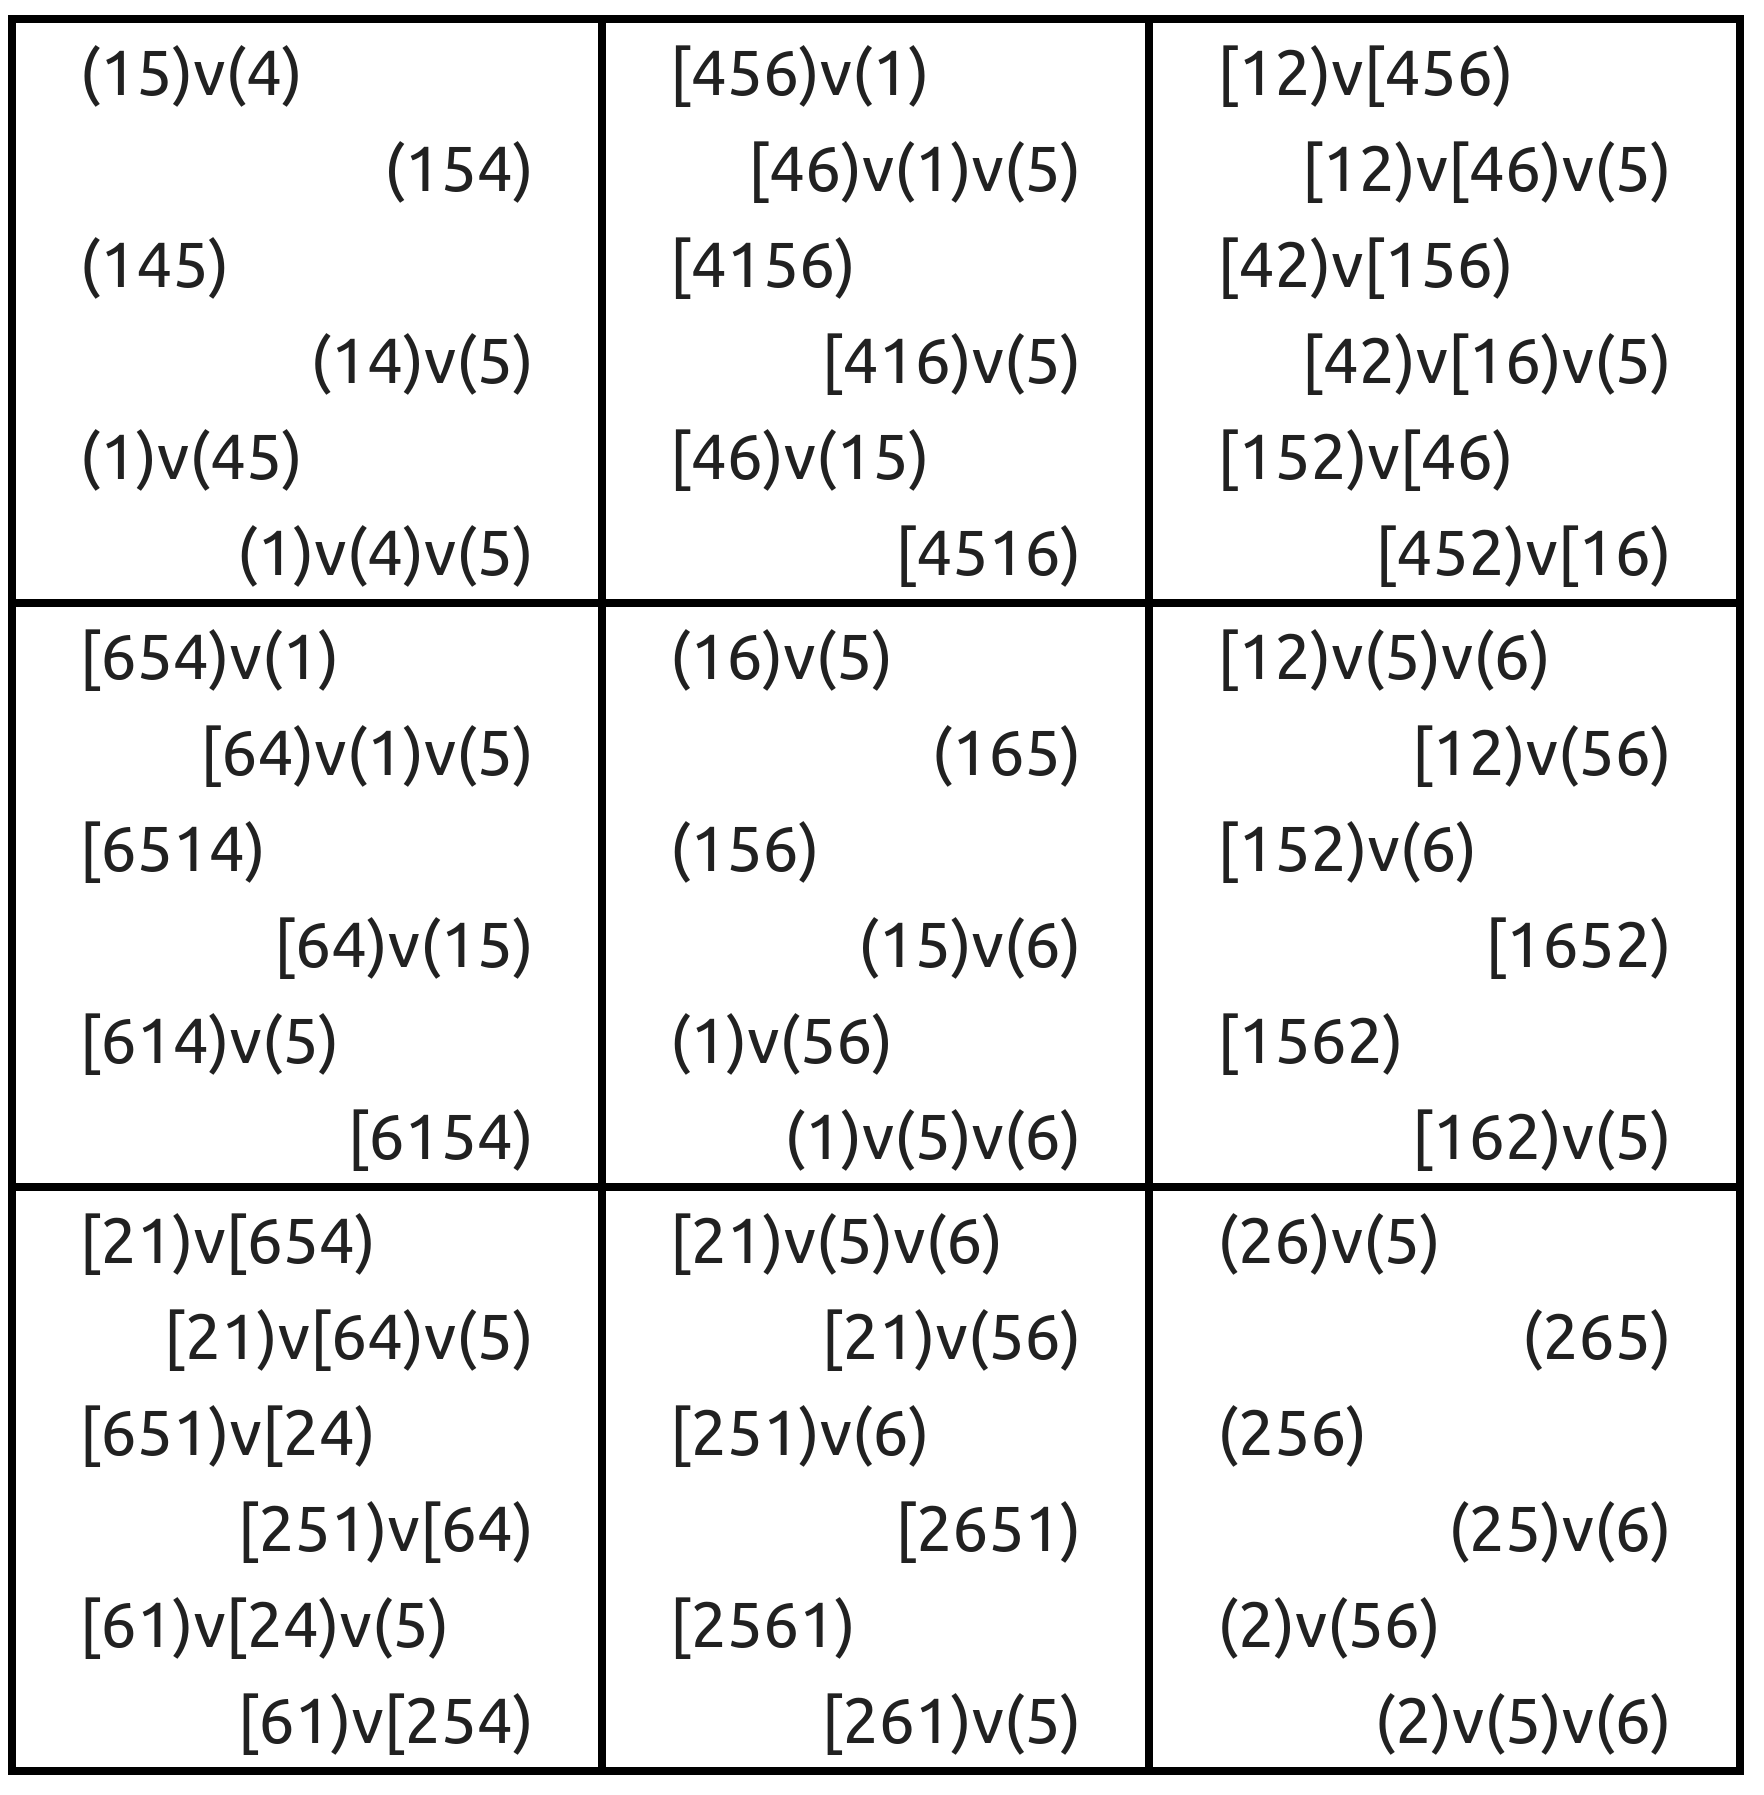
\includegraphics[scale=0.05]{images/x1/x1_3v_0e.png}
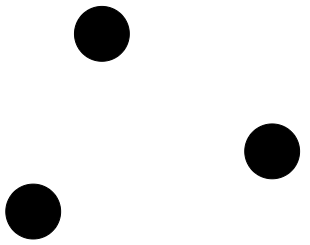
\includegraphics[scale=0.2]{images/x1/x1_3v_0e_vis.png}
\caption{$\mathcal{D}$-class of induced subgraph with 3 vertices and 0 edges (subgroup S3).}
\end{figure}

\begin{figure}[H]
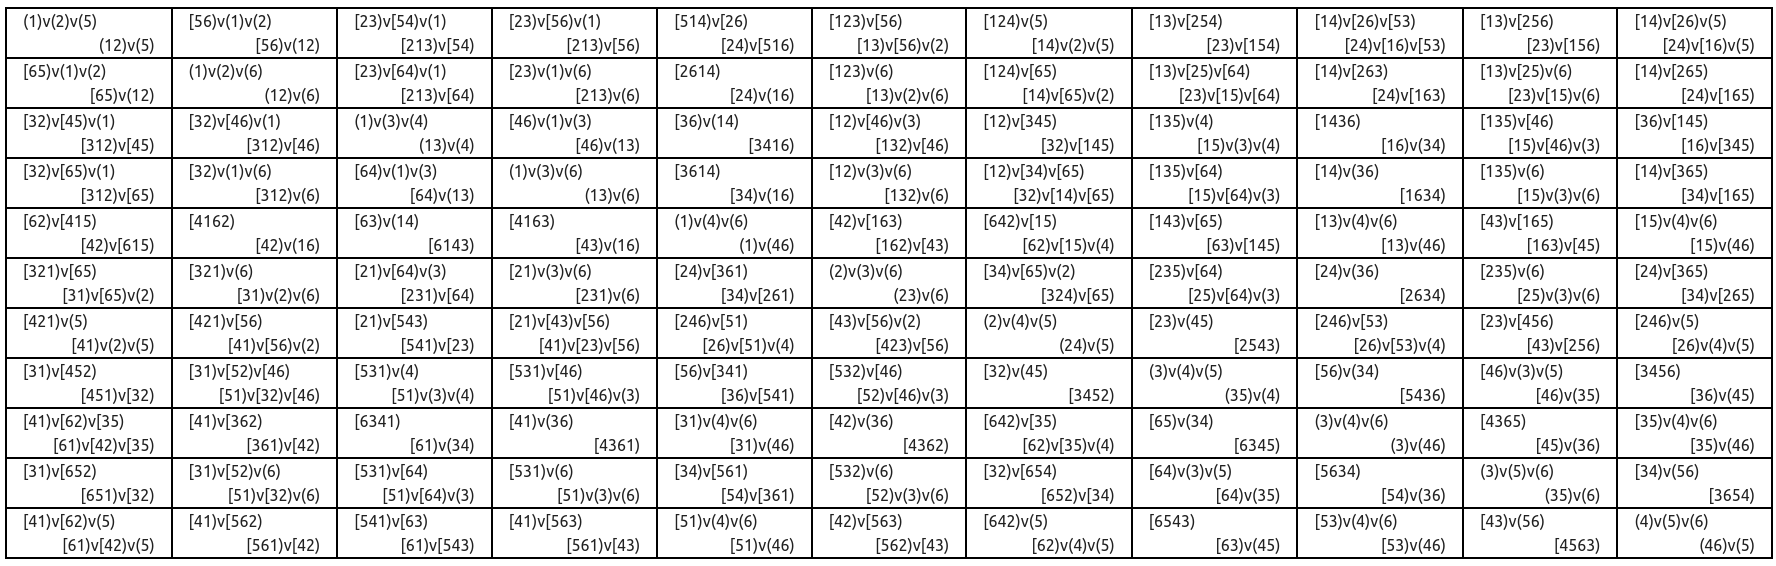
\includegraphics[width=\textwidth, keepaspectratio]{images/x1/x1_3v_1e.png}
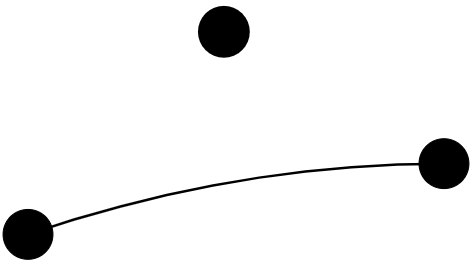
\includegraphics[scale=0.15]{images/x1/x1_3v_1e_vis.png}
\caption{$\mathcal{D}$-class of induced subgraph with 3 vertices and 1 edge (subgroup C2).}
\end{figure}

\begin{figure}[H]
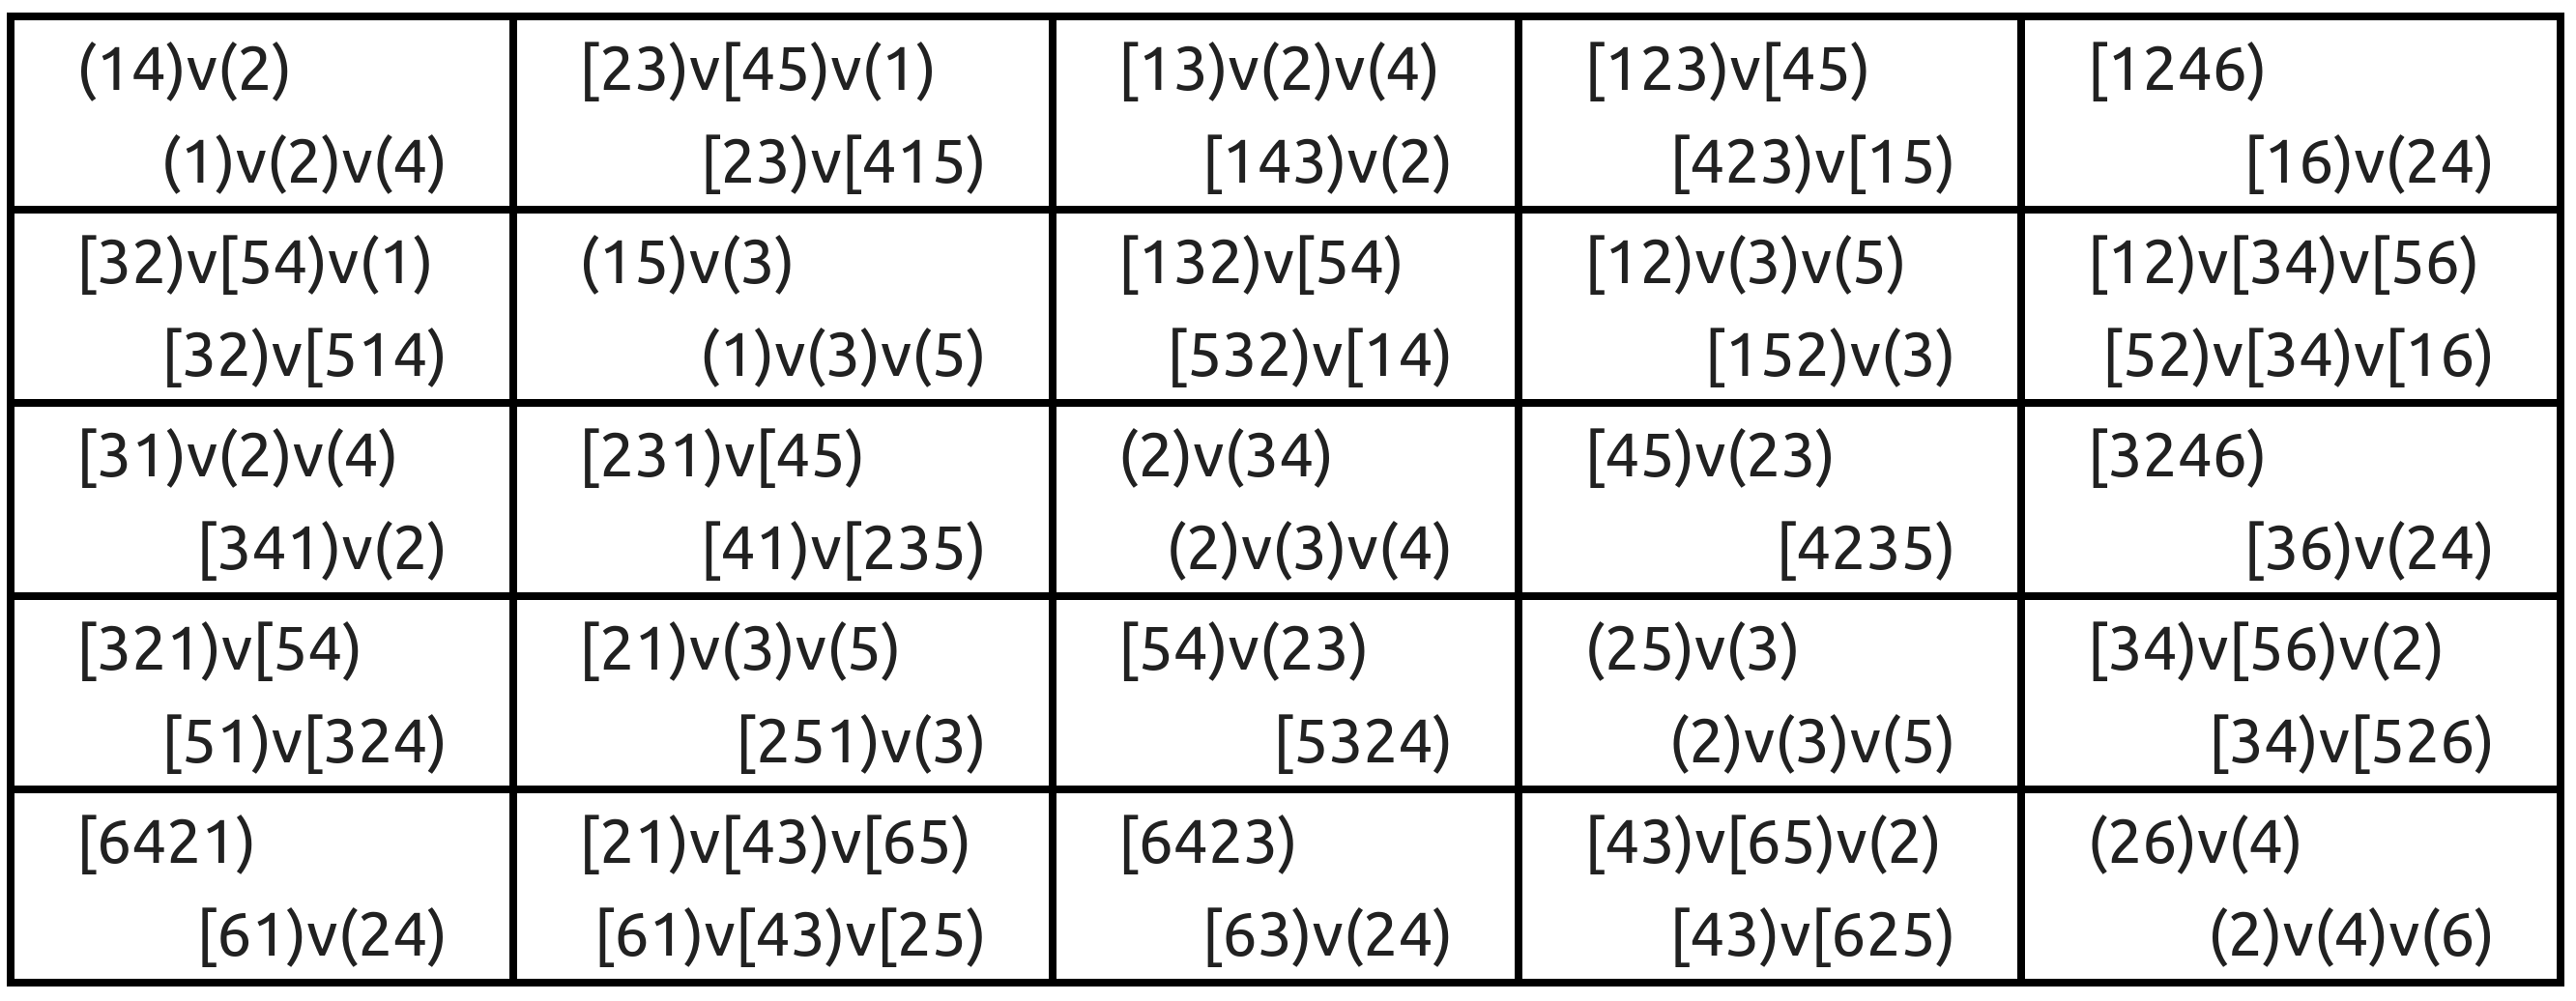
\includegraphics[scale=0.08]{images/x1/x1_3v_2e.png}
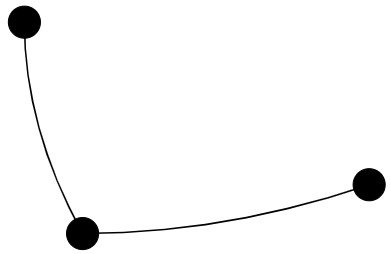
\includegraphics[scale=0.12]{images/x1/x1_3v_2e_vis.png}
\caption{$\mathcal{D}$-class of induced subgraph with 3 vertices and 2 edges (subgroup C2).}
\end{figure}

\begin{figure}[H]
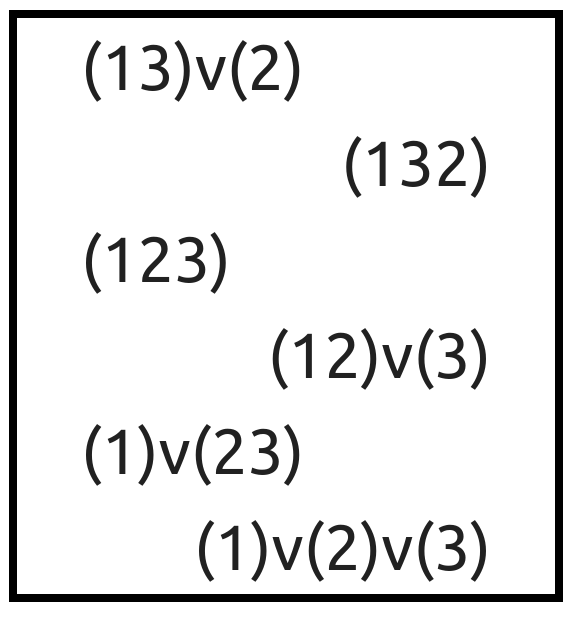
\includegraphics[scale=0.08]{images/x1/x1_3v_3e.png}
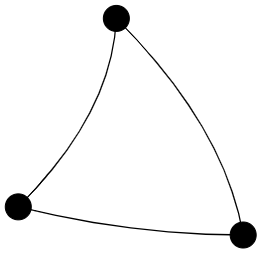
\includegraphics[scale=0.15]{images/x1/x1_3v_3e_vis.png}
\caption{$\mathcal{D}$-class of induced subgraph with 3 vertices and 3 edges (group S3).}
\end{figure}

\begin{figure}[H]
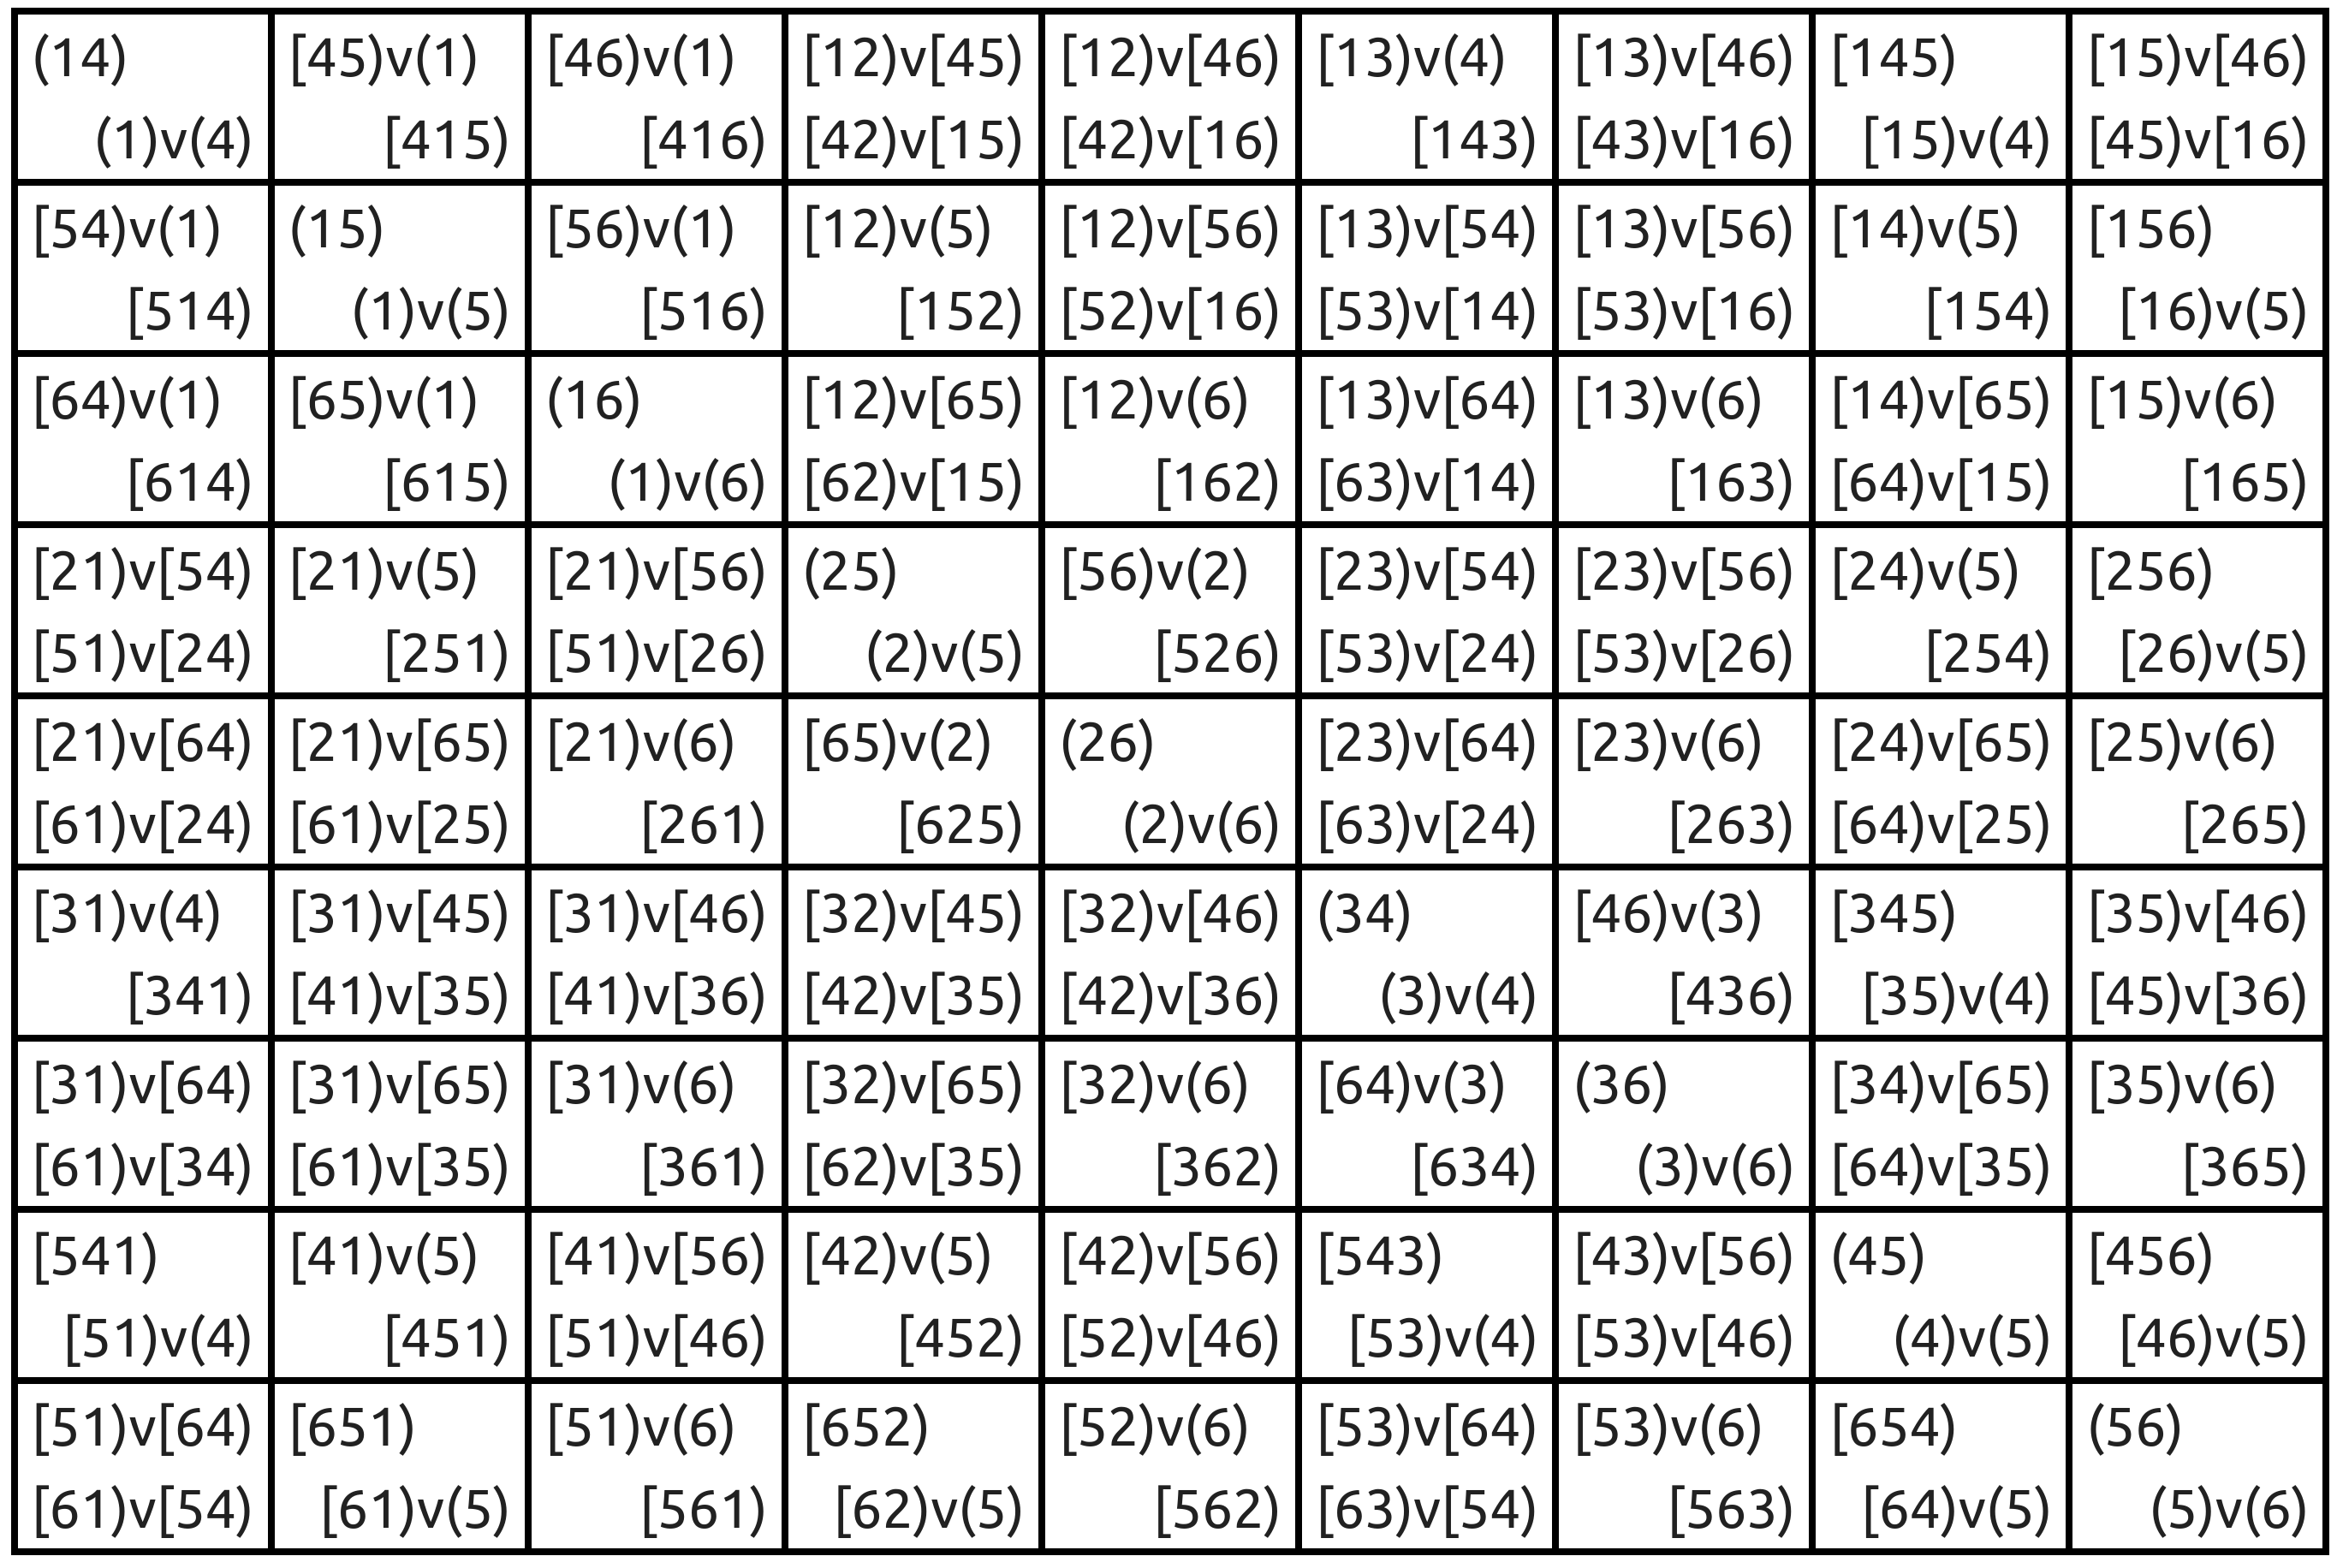
\includegraphics[scale=0.08]{images/x1/x1_2v_0e.png}
\caption{$\mathcal{D}$-class of induced subgraph with 2 vertices and 0 edges (subgroup C2).}
\end{figure}

\begin{figure}[H]
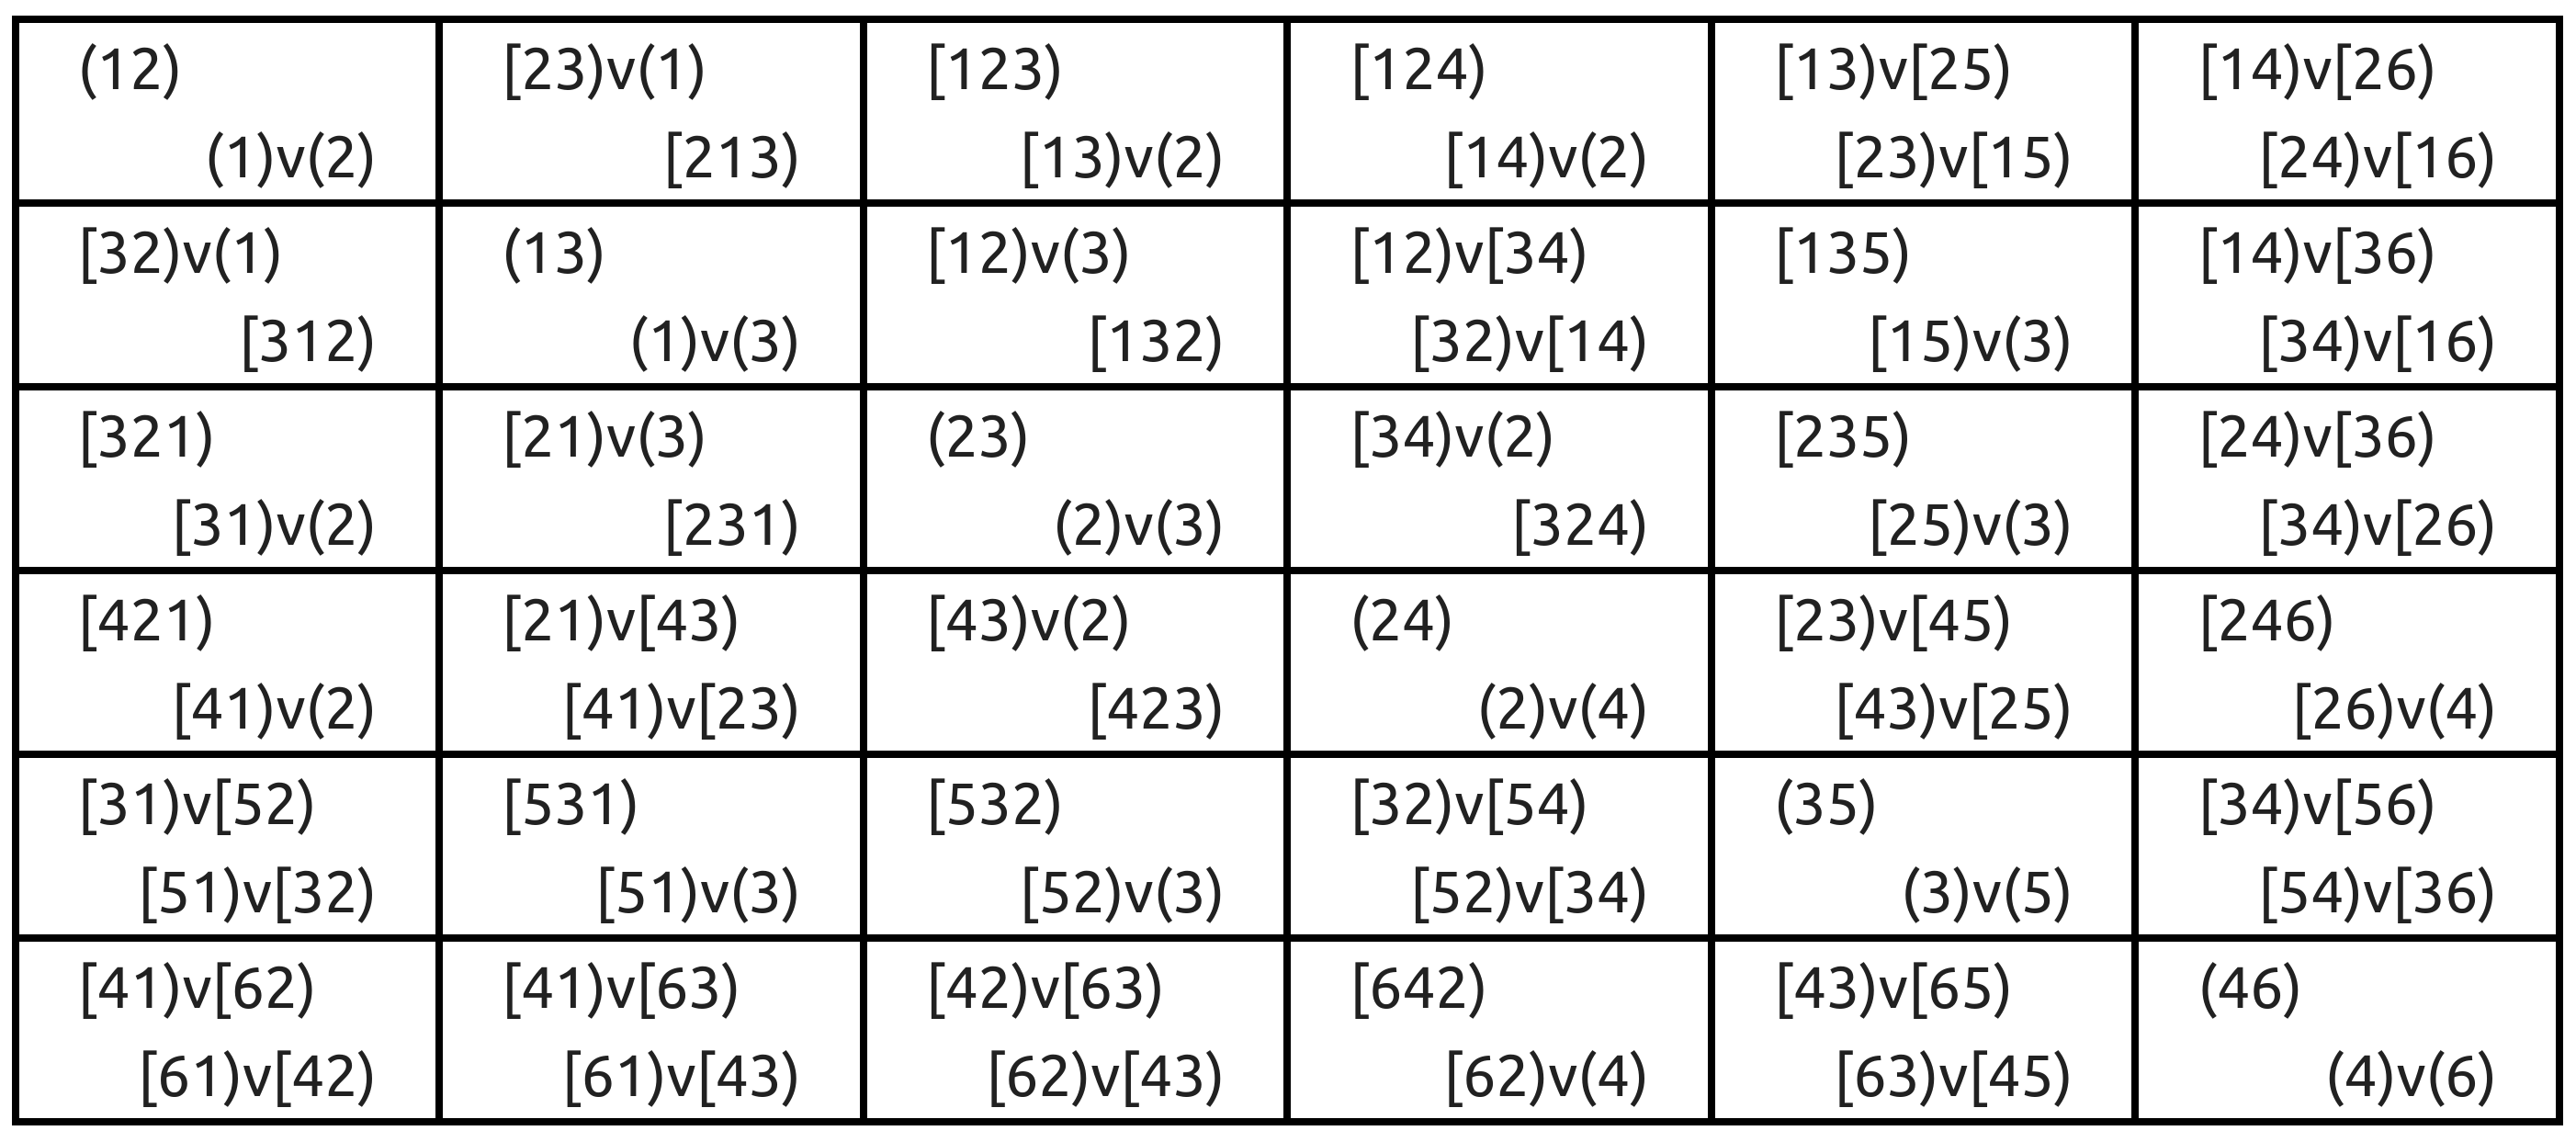
\includegraphics[scale=0.06]{images/x1/x1_2v_1e.png}
\caption{$\mathcal{D}$-class of induced subgraph with 2 vertices and 1 edge (subgroup C2).}
\end{figure}

\begin{figure}[H]
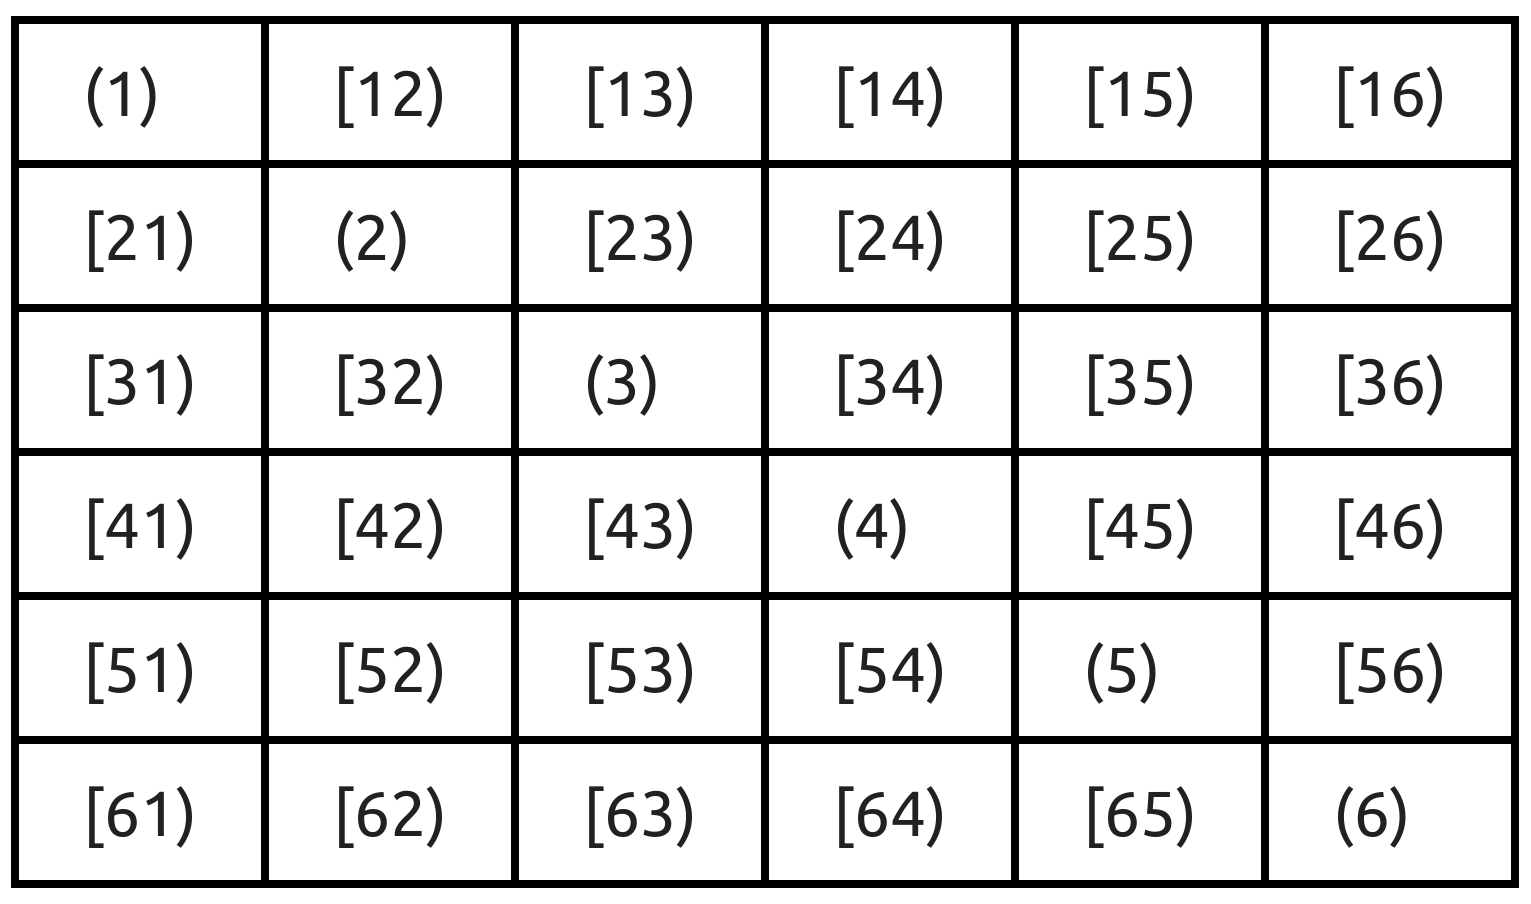
\includegraphics[scale=0.06]{images/x1/x1_1v_0e.png}
\caption{$\mathcal{D}$-class of induced subgraph with 1 vertex and 0 edges.}
\end{figure}

\section{Partial automorphism monoid of minimal asymmetric graph X9}

\begin{figure}[H]
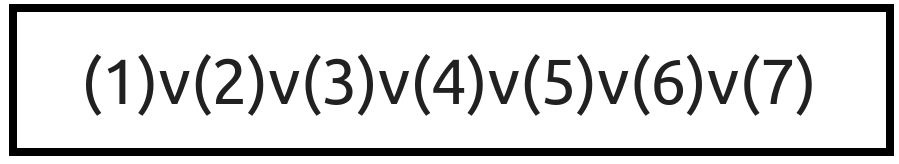
\includegraphics[scale=0.1]{images/x9/x9_7v_6e.png}
\caption{$\mathcal{D}$-class of induced subgraph with 7 vertices and 6 edges.}
\end{figure}

\begin{figure}[H]
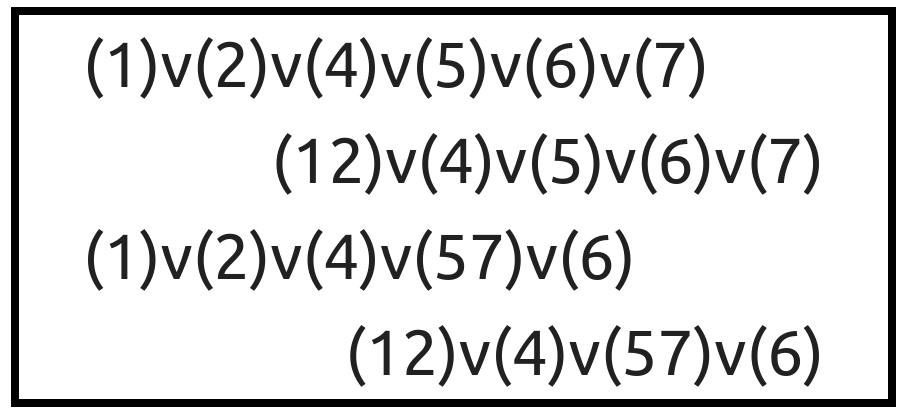
\includegraphics[scale=0.1]{images/x9/x9_6v_3e.png}
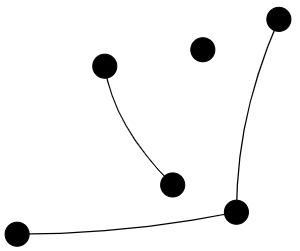
\includegraphics[scale=0.15]{images/x9/x9_6v_3e_vis.png}
\caption{$\mathcal{D}$-class of induced subgraph with 6 vertices and 3 edges (group C2xC2).}
\end{figure}

\begin{figure}[H]
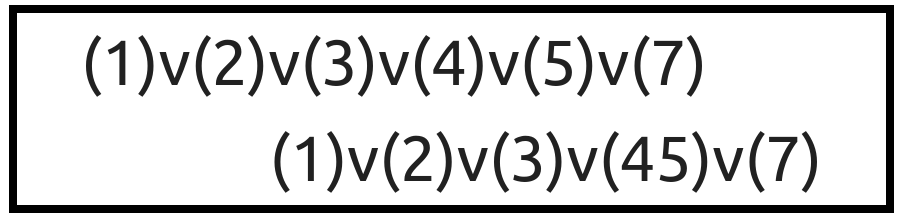
\includegraphics[scale=0.1]{images/x9/x9_6v_4e_1.png}
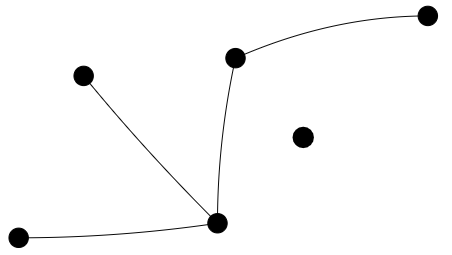
\includegraphics[scale=0.15]{images/x9/x9_6v_4e_1_vis.png}
\caption{$\mathcal{D}$-class of induced subgraph with 6 vertices and 4 edges (group C2).}
\end{figure}

\begin{figure}[H]
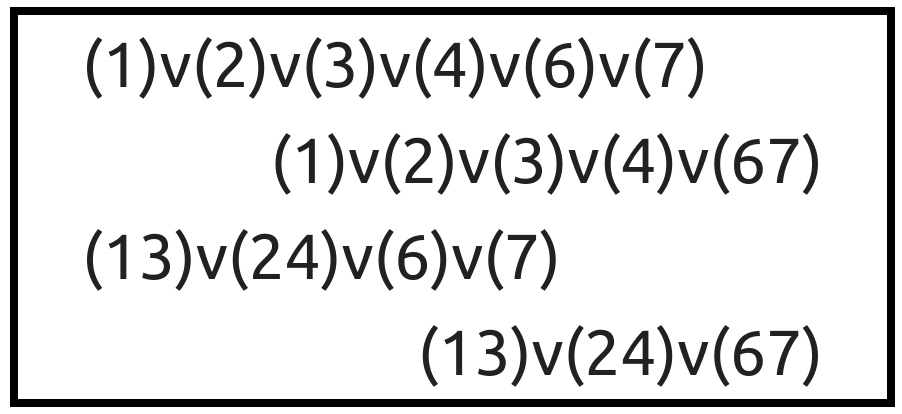
\includegraphics[scale=0.1]{images/x9/x9_6v_4e_2.png}
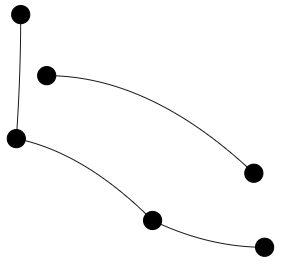
\includegraphics[scale=0.15]{images/x9/x9_6v_4e_2_vis.png}
\caption{$\mathcal{D}$-class of induced subgraph with 6 vertices and 4 edges (group C2xC2).}
\end{figure}

\begin{figure}[H]
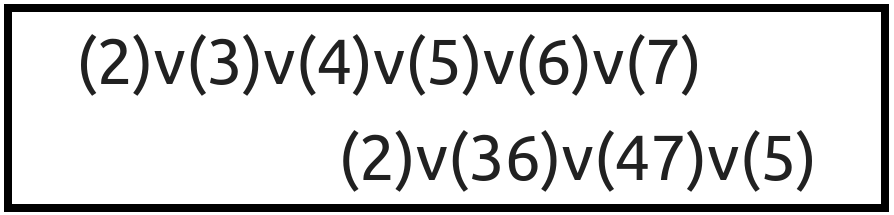
\includegraphics[scale=0.1]{images/x9/x9_6v_4e_3.png}
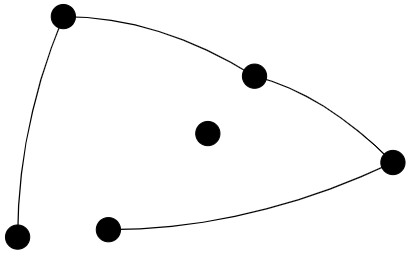
\includegraphics[scale=0.1]{images/x9/x9_6v_4e_3_vis.png}
\caption{$\mathcal{D}$-class of induced subgraph with 6 vertices and 4 edges (group C2).}
\end{figure}

\begin{figure}[H]
\includegraphics[scale=0.35]{images/x9/x9_6v_5e_1.png}
\includegraphics[scale=0.1]{images/x9/x9_6v_5e_1_vis.png}
\caption{$\mathcal{D}$-class of induced subgraph with 6 vertices and 5 edges (group C2).}
\end{figure}

\begin{figure}[H]
\includegraphics[scale=0.14]{images/x9/x9_6v_5e_2.png}
\includegraphics[scale=0.08]{images/x9/x9_6v_5e_2_vis.png}
\caption{$\mathcal{D}$-class of induced subgraph with 6 vertices and 5 edges (group C2).}
\end{figure}

\begin{figure}[H]
\includegraphics[scale=0.14]{images/x9/x9_6v_5e_3.png}
\includegraphics[scale=0.1]{images/x9/x9_6v_5e_3_vis.png}
\caption{$\mathcal{D}$-class of induced subgraph with 6 vertices and 5 edges (group C2).}
\end{figure}

\begin{figure}[H]
\includegraphics[scale=0.09]{images/x9/x9_5v_1e.png}
\includegraphics[scale=0.1]{images/x9/x9_5v_1e_vis.png}
\caption{$\mathcal{D}$-class of induced subgraph with 5 vertices and 1 edge (group D12).}
\end{figure}

\begin{figure}[H]
\includegraphics[scale=0.2]{images/x9/x9_5v_2e_1.png}
\includegraphics[scale=0.1]{images/x9/x9_5v_2e_1_vis.png}
\caption{$\mathcal{D}$-class of induced subgraph with 5 vertices and 2 edges (subgroup C2xC2).}
\end{figure}

\begin{figure}[H]
\includegraphics[scale=0.25]{images/x9/x9_5v_2e_2.png}
\includegraphics[scale=0.1]{images/x9/x9_5v_2e_2_vis.png}
\caption{$\mathcal{D}$-class of induced subgraph with 5 vertices and 2 edges (subgroup C2).}
\end{figure}

\begin{figure}[H]
\includegraphics[scale=0.09]{images/x9/x9_5v_3e_1.png}
\includegraphics[scale=0.1]{images/x9/x9_5v_3e_1_vis.png}
\caption{$\mathcal{D}$-class of induced subgraph with 5 vertices and 3 edges (group S3).}
\end{figure}

\begin{figure}[H]
\includegraphics[scale=0.2]{images/x9/x9_5v_3e_2.png}
\includegraphics[scale=0.1]{images/x9/x9_5v_3e_2_vis.png}
\caption{$\mathcal{D}$-class of induced subgraph with 5 vertices and 3 edges (subgroup C2xC2).}
\end{figure}

\begin{figure}[H]
\includegraphics[scale=0.2]{images/x9/x9_5v_3e_3.png}
\includegraphics[scale=0.1]{images/x9/x9_5v_3e_3_vis.png}
\caption{$\mathcal{D}$-class of induced subgraph with 5 vertices and 3 edges (subgroup C2).}
\end{figure}

\begin{figure}[H]
\includegraphics[scale=0.25]{images/x9/x9_5v_4e_1.png}
\includegraphics[scale=0.1]{images/x9/x9_5v_4e_1_vis.png}
\caption{$\mathcal{D}$-class of induced subgraph with 5 vertices and 4 edges (subgroup C2).}
\end{figure}

\begin{figure}[H]
\includegraphics[scale=0.25]{images/x9/x9_5v_4e_2.png}
\includegraphics[scale=0.1]{images/x9/x9_5v_4e_2_vis.png}
\caption{$\mathcal{D}$-class of induced subgraph with 5 vertices and 4 edges (subgroup C2).}
\end{figure}

\begin{figure}[H]
\includegraphics[scale=0.15]{images/x9/x9_4v_0e.png}
\includegraphics[scale=0.1]{images/x9/x9_4v_0e_vis.png}
\caption{$\mathcal{D}$-class of induced subgraph with 4 vertices and 0 edges (subgroup S4).}
\end{figure}

\begin{figure}[H]
\includegraphics[width=\textwidth,keepaspectratio]{images/x9/x9_4v_1e.png}
\includegraphics[scale=0.1]{images/x9/x9_4v_1e_vis.png}
\caption{$\mathcal{D}$-class of induced subgraph with 4 vertices and 1 edge (subgroup C2xC2).}
\end{figure}

\begin{figure}[H]
\includegraphics[scale=0.1]{images/x9/x9_4v_2e_1.png}
\includegraphics[scale=0.1]{images/x9/x9_4v_2e_1_vis.png}
\caption{$\mathcal{D}$-class of induced subgraph with 4 vertices and 2 edges (subgroup D8).}
\end{figure}

\begin{figure}[H]
\includegraphics[width=\textwidth,keepaspectratio]{images/x9/x9_4v_2e_2.png}
\includegraphics[scale=0.1]{images/x9/x9_4v_2e_2_vis.png}
\caption{$\mathcal{D}$-class of induced subgraph with 4 vertices and 2 edges (subgroup C2).}
\end{figure}

\begin{figure}[H]
\includegraphics[scale=0.1]{images/x9/x9_4v_3e_1.png}
\includegraphics[scale=0.1]{images/x9/x9_4v_3e_1_vis.png}
\caption{$\mathcal{D}$-class of induced subgraph with 4 vertices and 3 edges (group S3).}
\end{figure}

\begin{figure}[H]
\includegraphics[scale=0.2]{images/x9/x9_4v_3e_2.png}
\includegraphics[scale=0.1]{images/x9/x9_4v_3e_2_vis.png}
\caption{$\mathcal{D}$-class of induced subgraph with 4 vertices and 3 edges (subgroup C2).}
\end{figure}

\begin{figure}[H]
\includegraphics[width=\textwidth,keepaspectratio]{images/x9/x9_3v_0e.png}
\includegraphics[scale=0.1]{images/x1/x1_3v_0e_vis.png}
\caption{$\mathcal{D}$-class of induced subgraph with 3 vertices and 0 edges (subgroup S3).}
\end{figure}

\begin{figure}[H]
\includegraphics[width=\textwidth,keepaspectratio]{images/x9/x9_3v_1e.png}
\includegraphics[scale=0.1]{images/x1/x1_3v_1e_vis.png}
\caption{$\mathcal{D}$-class of induced subgraph with 3 vertices and 1 edge (subgroup C2).}
\end{figure}

\begin{figure}[H]
\includegraphics[scale=0.15]{images/x9/x9_3v_2e.png}
\includegraphics[scale=0.1]{images/x1/x1_3v_2e_vis.png}
\caption{$\mathcal{D}$-class of induced subgraph with 3 vertices and 2 edges (subgroup C2).}
\end{figure}

\begin{figure}[H]
\includegraphics[width=\textwidth, keepaspectratio]{images/x9/x9_2v_0e.png}
\caption{$\mathcal{D}$-class of induced subgraph with 2 vertices and 0 edges (subgroup C2).}
\end{figure}

\begin{figure}[H]
\includegraphics[scale=0.15]{images/x9/x9_2v_1e.png}
\caption{$\mathcal{D}$-class of induced subgraph with 2 vertices and 1 edge (subgroup C2).}
\end{figure}

\begin{figure}[H]
\includegraphics[scale=0.2]{images/x9/x9_1v_0e.png}
\caption{$\mathcal{D}$-class of induced subgraph with 1 vertex and 0 edges.}
\end{figure}

\end{appendices}

\end{document}